\documentclass[12pt]{article}	

\usepackage[margin=1in]{geometry}
\usepackage{amsmath,amssymb,amsthm}
\usepackage{caption}
\usepackage{subcaption}
\usepackage{graphicx}
\usepackage{url}
\usepackage{mathrsfs}
\newtheorem{theorem}{Theorem}
\newtheorem{notation}{Notation}
\newtheorem{claim}{Claim}
\newtheorem{lemma}{Lemma}
\newtheorem{definition}{Definition}
\renewcommand{\qedsymbol}{$\blacksquare$}
\newtheorem*{remark}{Remark}
\usepackage[utf8]{inputenc}

\usepackage{listings}
\usepackage{xcolor}

\definecolor{codegreen}{rgb}{0,0.6,0}
\definecolor{codegray}{rgb}{0.5,0.5,0.5}
\definecolor{codepurple}{rgb}{0.58,0,0.82}
\definecolor{backcolour}{rgb}{1,1,1}
\definecolor{grey}{rgb}{0.70, 0.70, 0.70}

\lstdefinestyle{mystyle}{
	backgroundcolor=\color{backcolour},   
	commentstyle=\color{grey},
	keywordstyle=\color{codepurple},
	numberstyle=\tiny\color{codegray},
	stringstyle=\color{codegreen},
	basicstyle=\ttfamily\footnotesize,
	breakatwhitespace=false,         
	breaklines=true,                 
	captionpos=b,                    
	keepspaces=true,                 
	numbers=left,                    
	numbersep=5pt,                  
	showspaces=false,                
	showstringspaces=false,
	showtabs=false,                  
	tabsize=2
}

\lstset{style=mystyle}


\begin{document}
	Arun Suresh
	\begin{center}
		Computational Physics 1 - Homework 8
	\end{center} 
	{\rule{\linewidth}{0.1mm} }

For my assignment, I chose to run the helix-pipe example that was provided in the Nek5000 example library for the class. \\
\indent The set up consists of fluid flowing through a helical pipe, which is a specific case of pipe-flow examples provided by Nek5000. The example was run three times, each run with a different value for the parameter lx1 which determined the order of the lagrange interpolating polynomial. The values chosen for the three runs were lx1 = 6, 7 and 8 (This means we have $N=5, 6$ and $7$ respectively). The three jobs were run on Harlow and the output was then copied to a remote computer, where VisIt was used in order to visualize the output. The visualizations are presented below. 
\\\\
\textbf{Mesh:}
	\begin{figure}[h]
	\centering
	\begin{subfigure}[h]{0.400\textwidth}
		\centering
		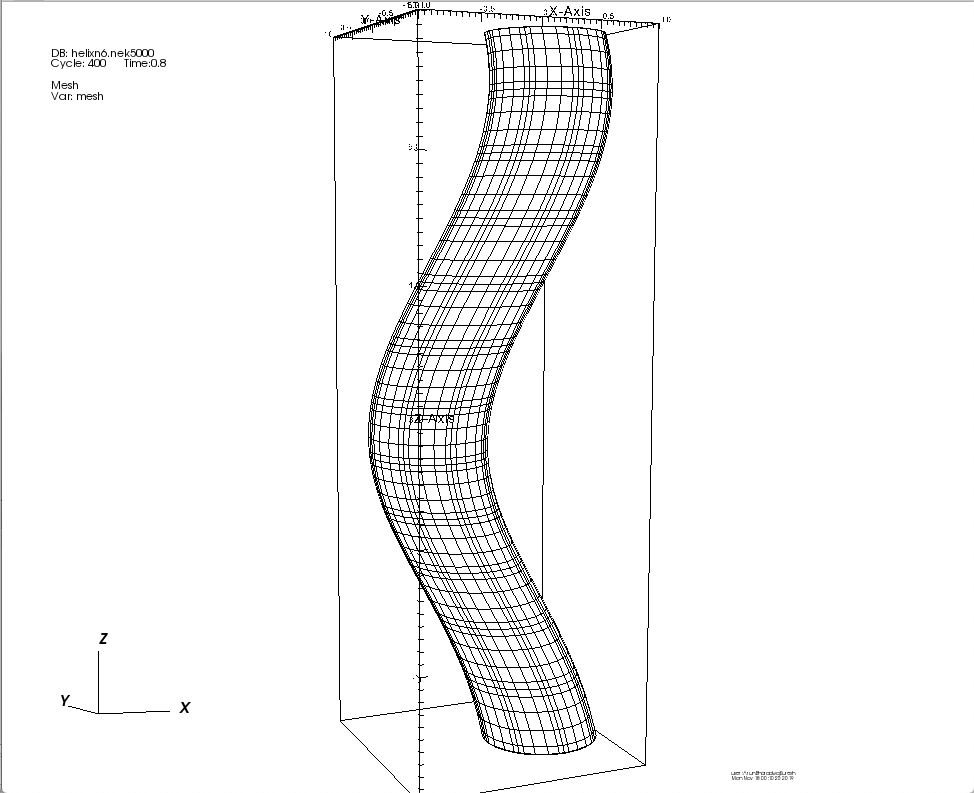
\includegraphics[width=\textwidth]{mesh6.png}
		\caption{N = 5}
	\end{subfigure}
	\begin{subfigure}[h]{0.400\textwidth}
		\centering
		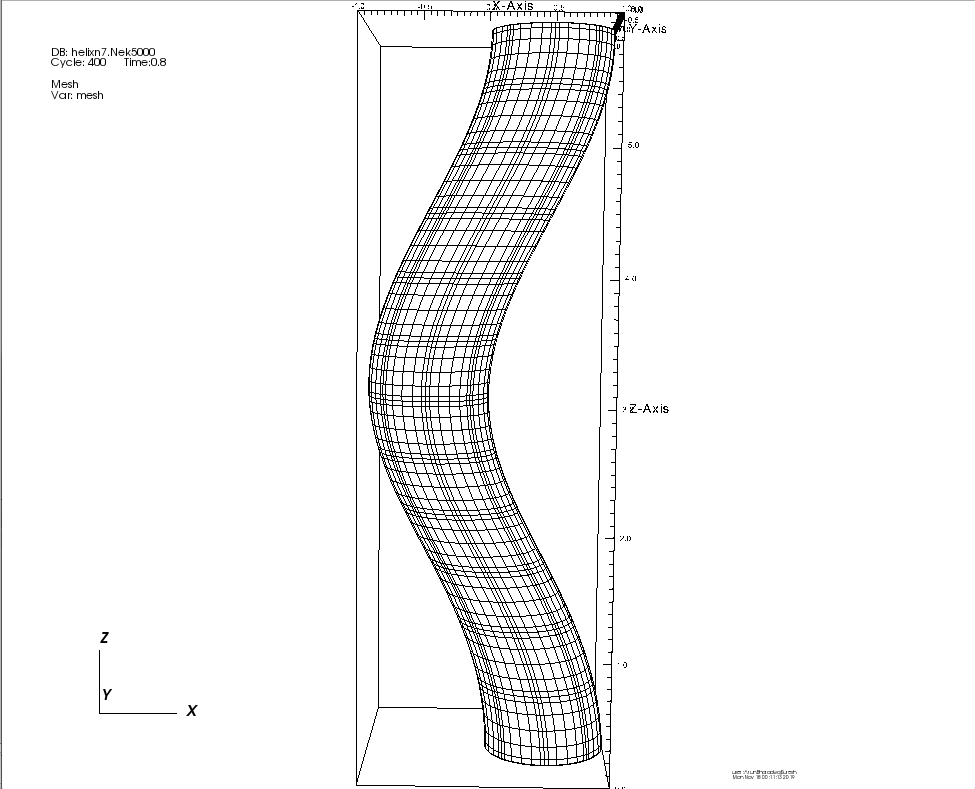
\includegraphics[width=\textwidth]{mesh7.png}
		\caption{N = 6}
	\end{subfigure}
	\begin{subfigure}[h]{0.400\textwidth}
		\centering
		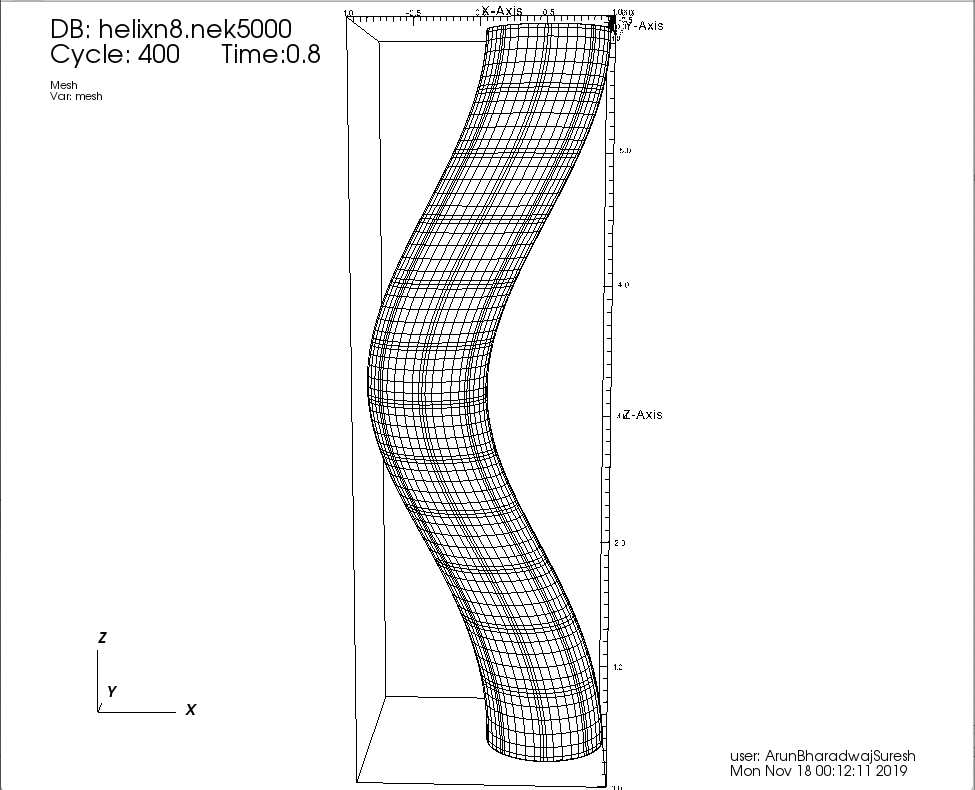
\includegraphics[width=\textwidth]{mesh8.png}
		\caption{N = 7}
	\end{subfigure}\\ 
\end{figure}\\
It is apparent that the mesh detailing improves as $N$ increases. This has a significant impact on the output that was observed. \\\\

The z-velocity of the flow was then observed as time progressed. This gives us direct insight into the distribution of the velocity profile along the pipe. This choice was made because the flow velocity is the easiest quantity to conceptualize and would enable us to verify theoretically if the results made sense. For this report, data from three different time frames (for the three cases) was compared. The time slices chosen are (in terms of clock cycles): 6000, 8800 and 11200 (12, 17.6, 22.4 seconds respectively) with each one being more insightful than the previous. The result (without mesh to avoid cluttering) as seen from the x-y crossection at the top of the pipe is presented below.\\
 
\noindent \textbf{z-velocity:}\\
\textbf{Clock: 6000}
\begin{figure}[h]
	\centering
	\begin{subfigure}[h]{0.400\textwidth}
		\centering
		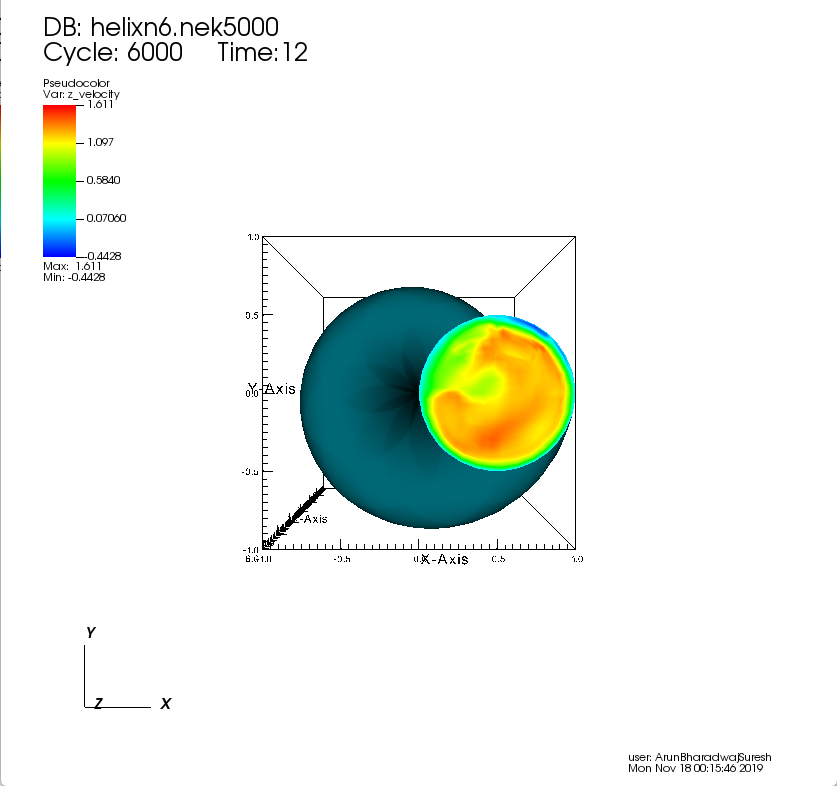
\includegraphics[width=\textwidth]{z6c6000.png}
		\caption{N = 5}
	\end{subfigure}
	\begin{subfigure}[h]{0.400\textwidth}
		\centering
		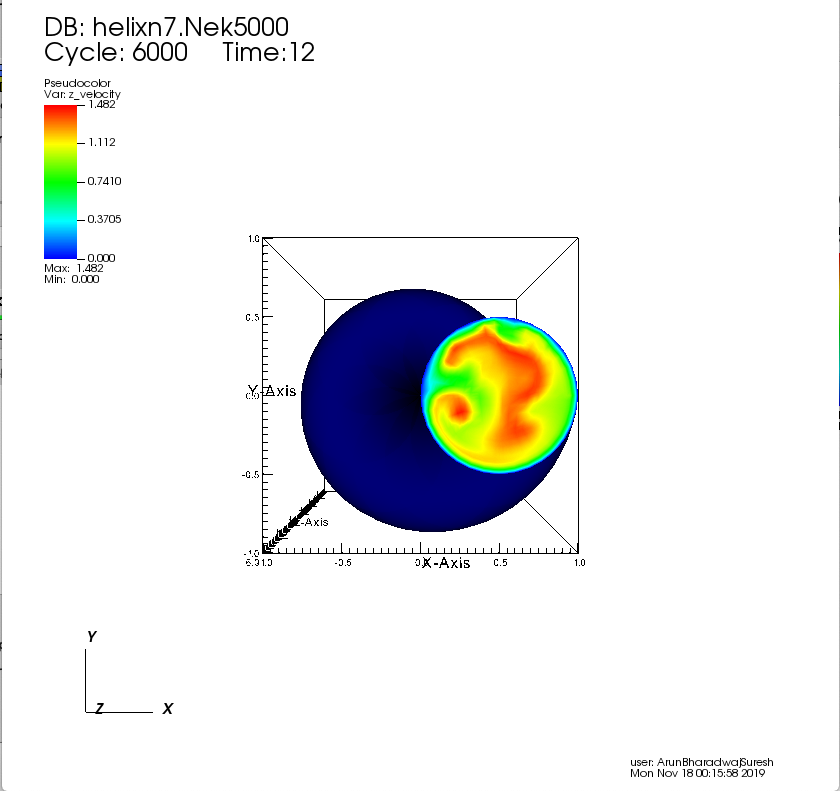
\includegraphics[width=\textwidth]{z7c6000.png}
		\caption{N = 6}
	\end{subfigure}
	\begin{subfigure}[h]{0.400\textwidth}
		\centering
		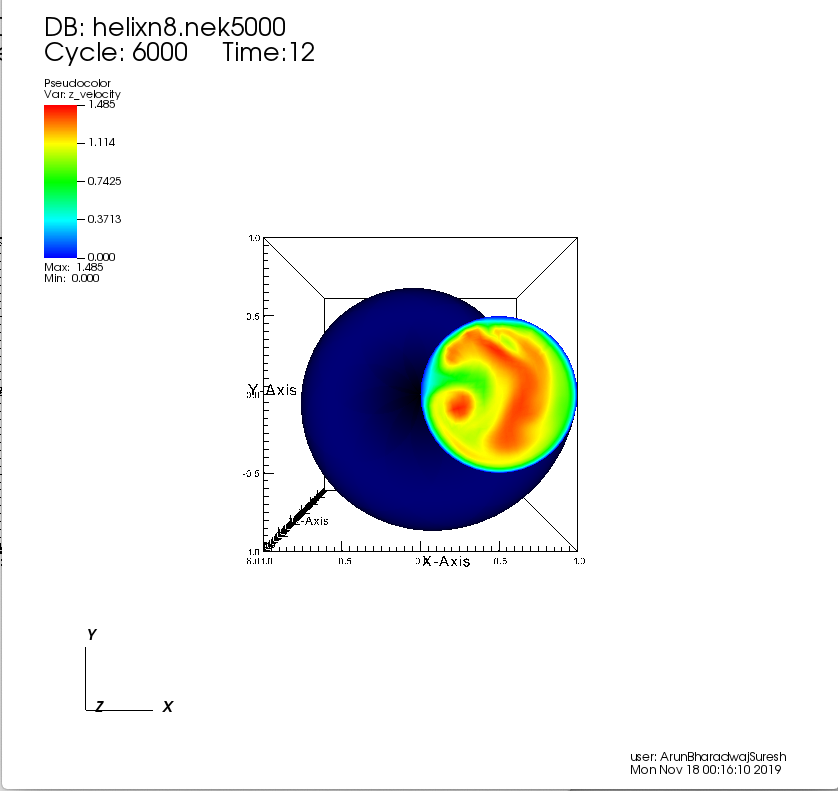
\includegraphics[width=\textwidth]{z8c6000.png}
		\caption{N = 7}
	\end{subfigure}\\ 
\end{figure}\\\\
Here, we observe that when $N=5$, we have that the flow closest to the pipe has a significant non-zero $z$-velocity which is clearly wrong; but as the order of the interpolating polynomial grows - the mesh is made dense and thus the error is not observed as expected. Moreover, the velocity profile acquires a lot more detail as $N$ increases - this is very apparent by noticing the how the shape of the high velocity areas increase in detail with $N$, and how the yellow-green areas obtain more defined shape. \\

\noindent \textbf{z-velocity:}\\
\textbf{Clock: 8800}
\begin{figure}[h]
	\centering
	\begin{subfigure}[h]{0.400\textwidth}
		\centering
		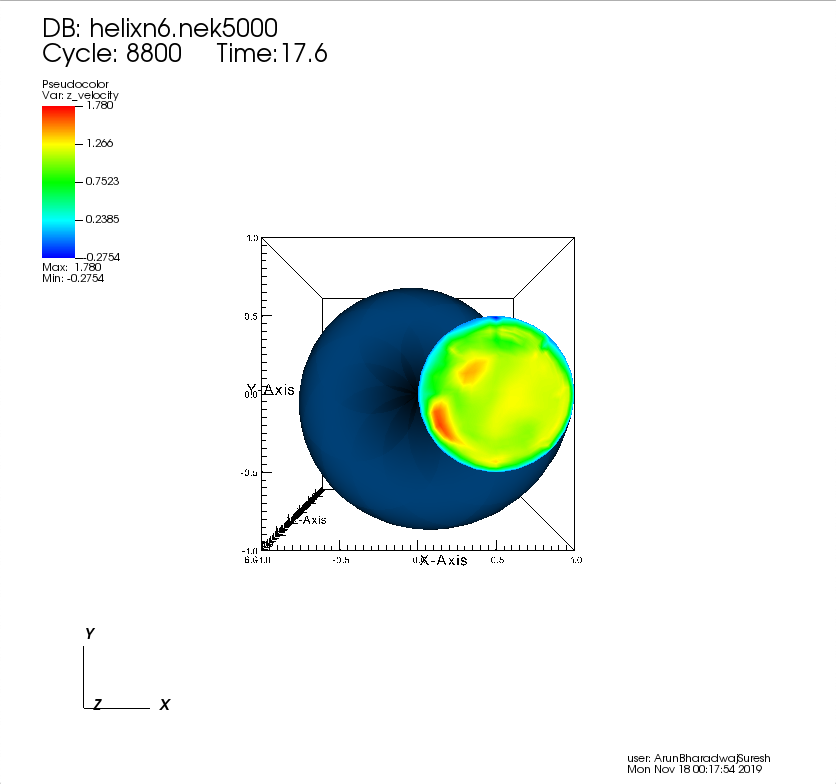
\includegraphics[width=\textwidth]{z6c8800.png}
		\caption{N = 5}
	\end{subfigure}
	\begin{subfigure}[h]{0.400\textwidth}
		\centering
		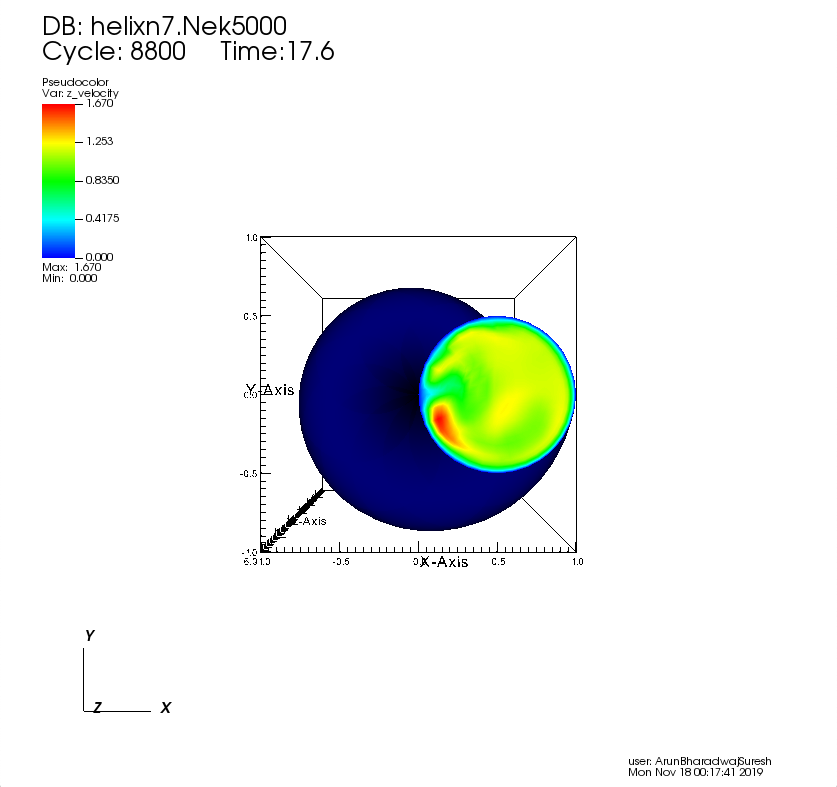
\includegraphics[width=\textwidth]{z7c8800.png}
		\caption{N = 6}
	\end{subfigure}
	\begin{subfigure}[h]{0.400\textwidth}
		\centering
		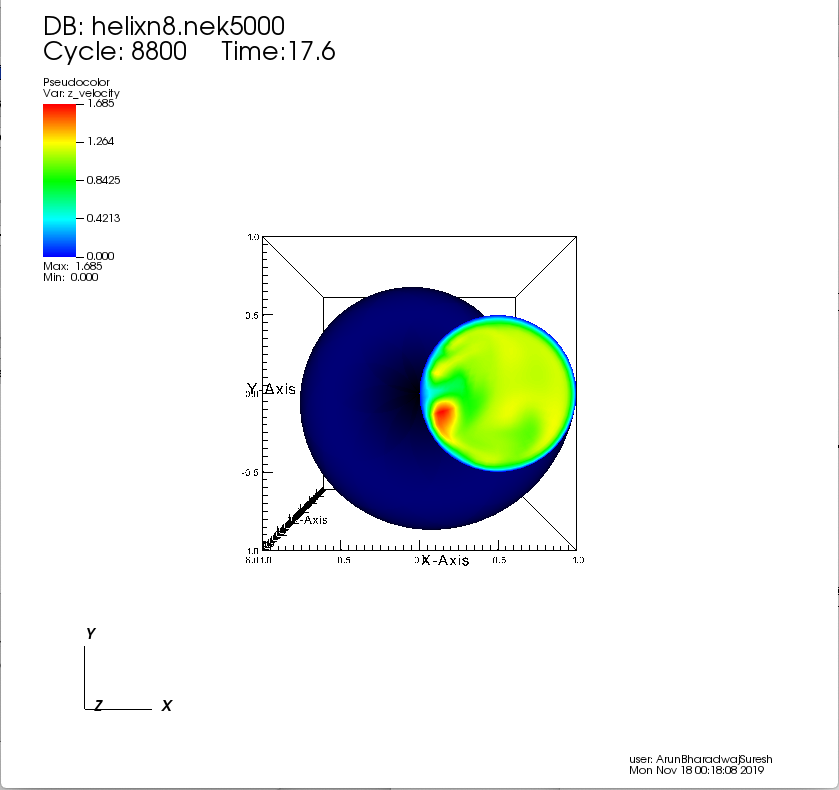
\includegraphics[width=\textwidth]{z8c8800.png}
		\caption{N = 7}
	\end{subfigure}\\ 
\end{figure}\\\\

Once again we notice a small non-zero velocity along the pipe when $N = 5$, and this error is eradicated when $N$ increases. But this time slice is interesting because it clearly highlights the difference in mesh structure between $N=6$ and $N=7$. Notice that the red high-velocity profile is well defined in shape and color when $N = 8$, whereas when $N=7$, we can see that it bleeds into nearby cells - creating an exaggeration in shape, and this exaggeration then leads to a dimming in the intensity of the color. Very similar comparisons can be made between $N=5$ and $N=6$. \\
\noindent \textbf{z-velocity:}\\
\textbf{Clock: 11200}
\begin{figure}[h]
	\centering
	\begin{subfigure}[h]{0.400\textwidth}
		\centering
		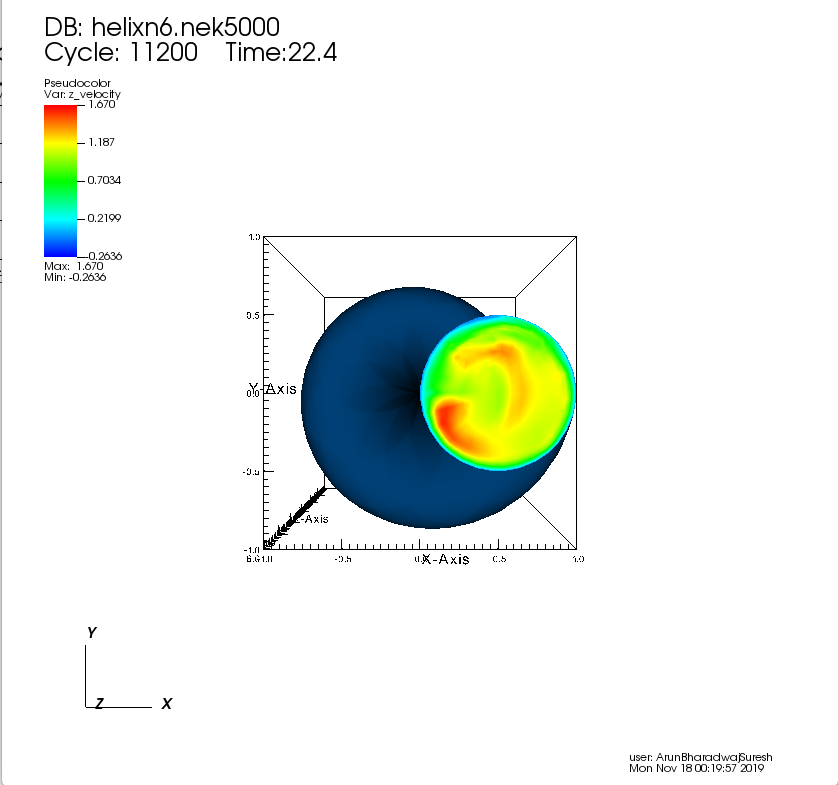
\includegraphics[width=\textwidth]{z6c11200.png}
		\caption{N = 5}
	\end{subfigure}
	\begin{subfigure}[h]{0.400\textwidth}
		\centering
		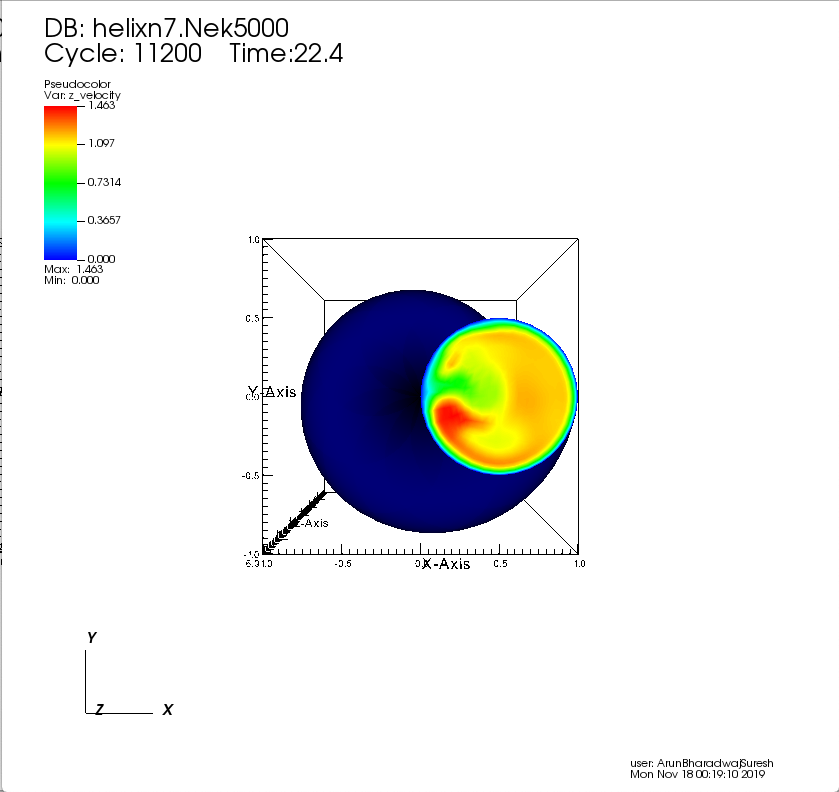
\includegraphics[width=\textwidth]{z7c11200.png}
		\caption{N = 6}
	\end{subfigure}
	\begin{subfigure}[h]{0.400\textwidth}
		\centering
		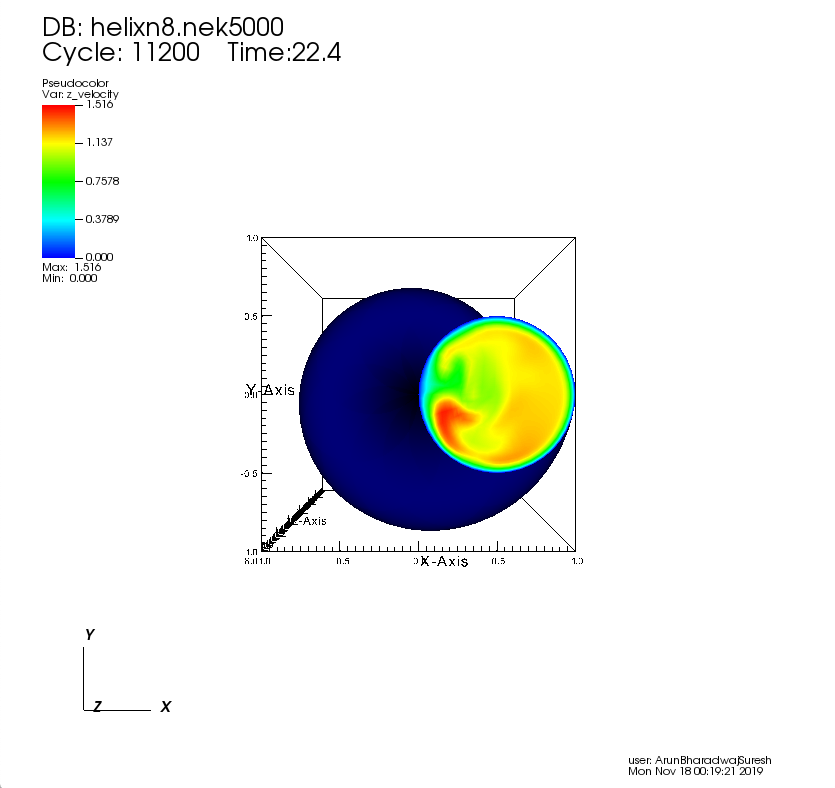
\includegraphics[width=\textwidth]{z8c11200.png}
		\caption{N = 7}
	\end{subfigure}\\ 
\end{figure}\\\\  

This is probably the best example that highlights all the differences we have observed. Once again we have edge effects and a very vague profile with $N=5$. The flow obtains more detail when $N=6$, and loses the issues with the edge effects, however, since the meshes are still big towards the center - the high velocity is a bit exaggerated. This is then fixed in $N=7$ where the profile obtains a better shape, and more detail is observed in the yellow-green phase as well. \\\\

\noindent \textbf{Understanding the flow}\\\\
I think the results that are observed makes physical sense. At first it seems odd that the velocity tends to be maximum off-center which is unusual for laminar flow. But this makes sense because the flow is happening in a helical pipe - and notice in figure 1 (mesh) that the center of the x-y crossection at the very bottom of the helix does not coincide with the center of the x-y crossection at the very top. Instead it is offset from the center due to the twist. Therefore it is natural to expect the high velocity flow at the bottom of the pipe to skew away from the center and towards the walls of the pipe creating a high velocity profile that is off-centered at the very top. In fact, this effect was visualized using VisIt where the velocity vectors were drawn at each mesh in the pipe at clock cycle 11200. The results are presented below\\\\

\noindent \textbf{velocity:}\\
\textbf{Clock: 11200}
\begin{figure}[h]
	\centering
	\begin{subfigure}[h]{0.400\textwidth}
		\centering
		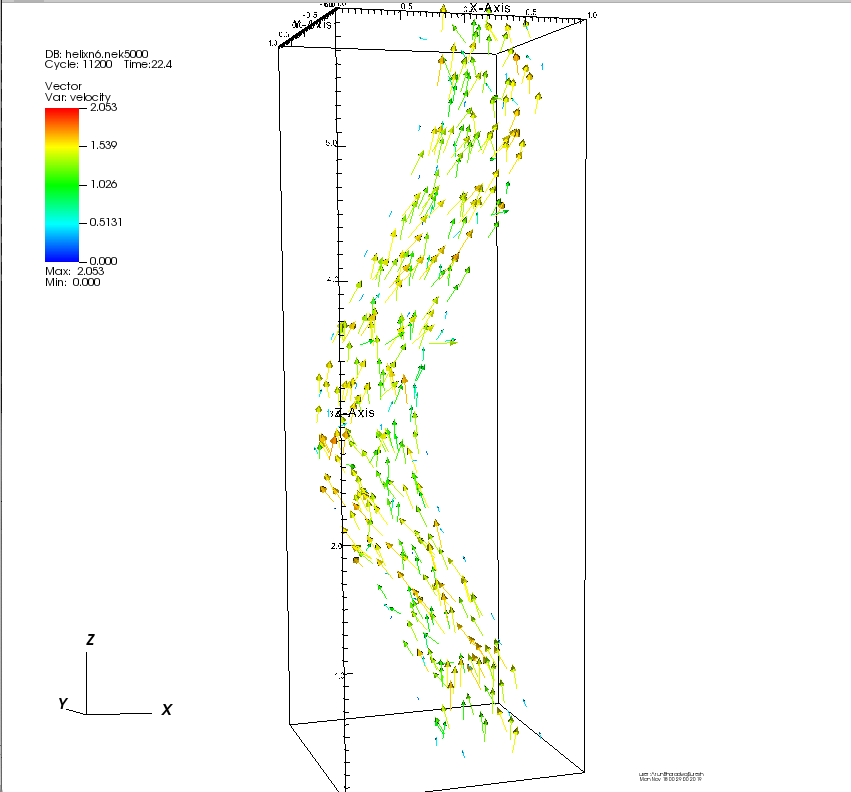
\includegraphics[width=\textwidth]{vector6_11200.png}
		\caption{N = 5}
	\end{subfigure}
	\begin{subfigure}[h]{0.400\textwidth}
		\centering
		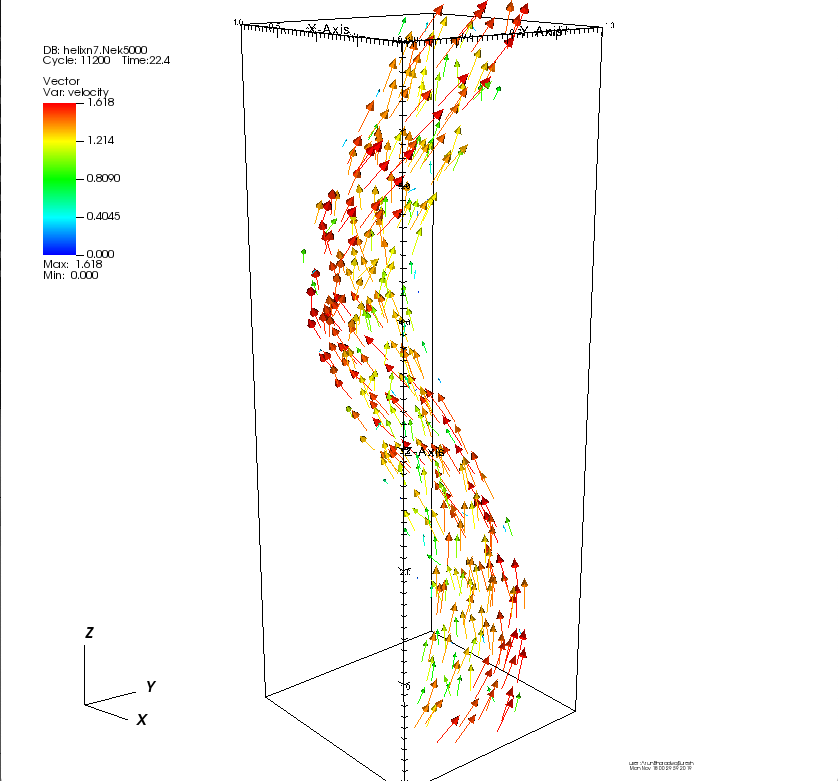
\includegraphics[width=\textwidth]{vector7_11200.png}
		\caption{N = 6}
	\end{subfigure}
	\begin{subfigure}[h]{0.400\textwidth}
		\centering
		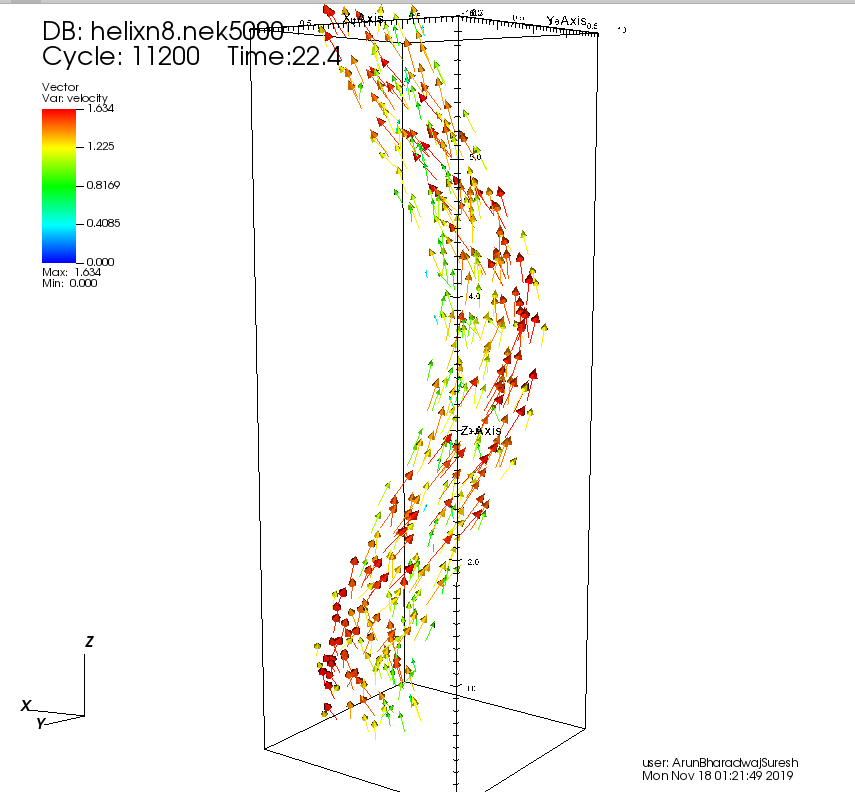
\includegraphics[width=\textwidth]{vector8_11200.png}
		\caption{N = 7}
	\end{subfigure}\\ 
\end{figure}\\
It is once again apparent that the results get better as $N$ increases (notice how the high-velocities become well defined in position and magnitude as $N$ increases). But most importantly, the arrows provide evidence for our claim (Notice the bottom of $N=7$) that centered high velocity flow skews off-center due to the helical twist. 



\end{document}